\documentclass{article}
\usepackage[]{graphicx}
\usepackage[]{color}
\usepackage{hyperref}

\graphicspath{ {./images/} }
% maxwidth is the original width if it is less than linewidth
% otherwise use linewidth (to make sure the graphics do not exceed the margin)
\makeatletter
\def\maxwidth{ %
  \ifdim\Gin@nat@width>\linewidth
    \linewidth
  \else
    \Gin@nat@width
  \fi
}
\makeatother

\definecolor{fgcolor}{rgb}{0.345, 0.345, 0.345}
\newcommand{\hlnum}[1]{\textcolor[rgb]{0.686,0.059,0.569}{#1}}%
\newcommand{\hlstr}[1]{\textcolor[rgb]{0.192,0.494,0.8}{#1}}%
\newcommand{\hlcom}[1]{\textcolor[rgb]{0.678,0.584,0.686}{\textit{#1}}}%
\newcommand{\hlopt}[1]{\textcolor[rgb]{0,0,0}{#1}}%
\newcommand{\hlstd}[1]{\textcolor[rgb]{0.345,0.345,0.345}{#1}}% 
\newcommand{\hlkwa}[1]{\textcolor[rgb]{0.161,0.373,0.58}{\textbf{#1}}}%
\newcommand{\hlkwb}[1]{\textcolor[rgb]{0.69,0.353,0.396}{#1}}%
\newcommand{\hlkwc}[1]{\textcolor[rgb]{0.333,0.667,0.333}{#1}}%
\newcommand{\hlkwd}[1]{\textcolor[rgb]{0.737,0.353,0.396}{\textbf{#1}}}%
\let\hlipl\hlkwb

\usepackage{framed}
\makeatletter
\newenvironment{kframe}{%
 \def\at@end@of@kframe{}%
 \ifinner\ifhmode%
  \def\at@end@of@kframe{\end{minipage}}%
  \begin{minipage}{\columnwidth}%
 \fi\fi%
 \def\FrameCommand##1{\hskip\@totalleftmargin \hskip-\fboxsep
 \colorbox{shadecolor}{##1}\hskip-\fboxsep
     % There is no \\@totalrightmargin, so:
     \hskip-\linewidth \hskip-\@totalleftmargin \hskip\columnwidth}%
 \MakeFramed {\advance\hsize-\width
   \@totalleftmargin\z@ \linewidth\hsize
   \@setminipage}}%
 {\par\unskip\endMakeFramed%
 \at@end@of@kframe}
\makeatother

\definecolor{shadecolor}{rgb}{.97, .97, .97}
\definecolor{messagecolor}{rgb}{0, 0, 0}
\definecolor{warningcolor}{rgb}{1, 0, 1}
\definecolor{errorcolor}{rgb}{1, 0, 0}
\newenvironment{knitrout}{}{} % an empty environment to be redefined in TeX

\usepackage{alltt}
\usepackage{listings}

\definecolor{mygreen}{rgb}{0,0.6,0}
\definecolor{mygray}{rgb}{0.5,0.5,0.5}
\definecolor{mymauve}{rgb}{0.58,0,0.82}

\lstset{ 
  backgroundcolor=\color{white},   % choose the background color; you must add \usepackage{color} or \usepackage{xcolor}; should come as last argument
  basicstyle=\footnotesize,        % the size of the fonts that are used for the code
  breakatwhitespace=false,         % sets if automatic breaks should only happen at whitespace
  breaklines=true,                 % sets automatic line breaking
  captionpos=,                    % sets the caption-position to bottom
  commentstyle=\color{mygreen},    % comment style
  deletekeywords={...},            % if you want to delete keywords from the given language
  escapeinside={\%*}{*)},          % if you want to add LaTeX within your code
  extendedchars=true,              % lets you use non-ASCII characters; for 8-bits encodings only, does not work with UTF-8
  firstnumber=1,                % start line enumeration with line 1000
  frame=single,	                   % adds a frame around the code
  keepspaces=true,                 % keeps spaces in text, useful for keeping indentation of code (possibly needs columns=flexible)
  keywordstyle=\color{blue},       % keyword style
  language=Python,                 % the language of the code
  morekeywords={*,...},            % if you want to add more keywords to the set
  numbers=left,                    % where to put the line-numbers; possible values are (none, left, right)
  numbersep=5pt,                   % how far the line-numbers are from the code
  numberstyle=\tiny\color{mygray}, % the style that is used for the line-numbers
  rulecolor=\color{black},         % if not set, the frame-color may be changed on line-breaks within not-black text (e.g. comments (green here))
  showspaces=false,                % show spaces everywhere adding particular underscores; it overrides 'showstringspaces'
  showstringspaces=false,          % underline spaces within strings only
  showtabs=false,                  % show tabs within strings adding particular underscores
  stepnumber=1,                    % the step between two line-numbers. If it's 1, each line will be numbered
  stringstyle=\color{mymauve},     % string literal style
  tabsize=2,	                   % sets default tabsize to 2 spaces
  title=\lstname                   % show the filename of files included with \lstinputlisting; also try caption instead of title
}

\title{Connecting Sensors to Pi}
\author{Kyle McCarty and Marc Los Huertos\footnote{Acknowledgments: Much of the project is based on summer research conducted by Anna Burns.}}
\IfFileExists{upquote.sty}{\usepackage{upquote}}{}
\begin{document}
\maketitle
\tableofcontents

\section{Introduction}


\subsection{What is particulate matter?}

PM stands for particulate matter (also called particle pollution). Particulate Matter is a mixture of solid particles and liquid droplets found in the air. Some particles, such as dust, dirt, soot, or smoke, are large or dark enough to be seen with the naked eye. Others are so small they can only be detected using an electron microscope.

Particle pollution can be classified by size:

\begin{description}
  \item[PM10] inhalable particles, with diameters that are generally 10 micrometers and smaller; and

  \item[PM2.5] fine inhalable particles, with diameters that are generally 2.5 micrometers and smaller.
  
NOTE: The average human hair is about 70 micrometers in diameter --- making it 30 times larger than the largest fine particle.

\end{description}

\section{PMS5003 Particulate matter sensor}

\subsection{Sensor Purchase}
The Digital Particle Concentration Laser Sensor Plantower PMS5003 PM2.5 PM10 is produced in China. With 25 purchases, they cost about \$23 each.

\subsection{Sensor Construction and Operation}


\subsection{Sensor IO}

This sensor comes with eight female-to-female connectors as well as an adapter for the Raspberry Pi, and a connector for the Raspberry Pi and the adapter itself.  

\subsection{Wiring}

\begin{enumerate}
  \item Begin by connecting the sensor to the adapter. Take the colorful wires with white blocks on either end and attach them to both the sensor and the small adapter board; they attach with the ``shiny'' side up, and you need to give them quite a push to get them to go in fully. They should be snug, and not at all loose.

  \item Next, connect the adapter to the Raspberry Pi.  Separate four of the female-to-female connectors (the ones with the black rectangles on either end) and attach one of the ends to the TXD, RXD, GND and VCO terminals on the adapter (these correspond to the 4th, 5th, 7th, and 8th terminals from the top).  

\begin{itemize}
  \item Connect the wire attached to the VCC terminal to PIN 2 on the Raspberry Pi -- or connect to the 5V rail on the breadboad.

  \item Connect the wire attached to the GND terminal to PIN 9 on the Raspberry Pi -- or connect to the ground rail on the breadboard. 

  \item Connect the wire attached to the RXD terminal to PIN 8 on the Raspberry Pi. 

  \item Connect the wire attached to the TXD terminal to PIN 10 on the Raspberry Pi.
\end{itemize}

\item Double check the wiring with the following images

\end{enumerate}


\subsection{Code and Testing}

\begin{enumerate}
  \item Connect your Pi to power and PMS5003 fan should start.
  \item VNC to the Pi.
  \item Check to make sure that it is working. If not shut the Pi down (via the command `sudo shutdown' and check the wiring. 

\item Enter ``sudo raspi-config".

\item Select Option 5 (``Interfacing Options").

\item Enable ARM I2C by selecting it in this menu and then pressing Yes.

\item Then to enable Serial, select Option 5 (``Interfacing Options") again and choose Serial on the menu. 

\item A window will pop up asking, ``would you like a login shell to be accessible over serial?", and the answer is NO.

\item Next, a window will pop up asking, ``Would you like the serial port hardware to be enabled?", this time say YES, and exit the window.

\item Click Finish, you may be prompted to reboot, and select YES.

\item We will also need to download a pre-made communication tool.  Using the command window, type ``

\end{enumerate}

\subsection{Python Code}

We have made the code available on the EJnPi Respository, so you can download it directly from the web onto your Pi or follow the steps below:

\begin{enumerate}

\item Using the Pi's webbrowser, navigate to \href{https://github.com/marclos/EJnPi/tree/master/code}{the EJnPI Respository}. 

\item When you can get the the files and ``Blame'' in Github to view the Air\_quality\_code\_v2.py, then click to save on the home directory.

Then open Thorny and load the file.

\lstinputlisting{../code/Air_quality_code_v2.py}

\item Open the file using Thorny and hit run. You should see the results being displayed in the lower window.


%5.  Now within the main shell, type "python3 pms5003.py". When I submitted the text, I got one of two responses -- some error, usually about some indentation problem that took way too long to sort out OR it seem to quietly be in standby mode. I think it was sending the program to my Pi, perhaps compiling and sending the commands to the sensor.  

\item It should release a reading of the different measurements specified at intervals of 60 seconds, and compile the data into a CSV file.

\end{enumerate}
\section{MQ Sensors}

\subsection{Additional Sensors}

We have provided the electronics to evaluate other air quality parameters using MQ Sensors. You can read about how these sensors work and a list of types of sensors in this \href{http://github...}{sensor guide}.

\begin{figure}
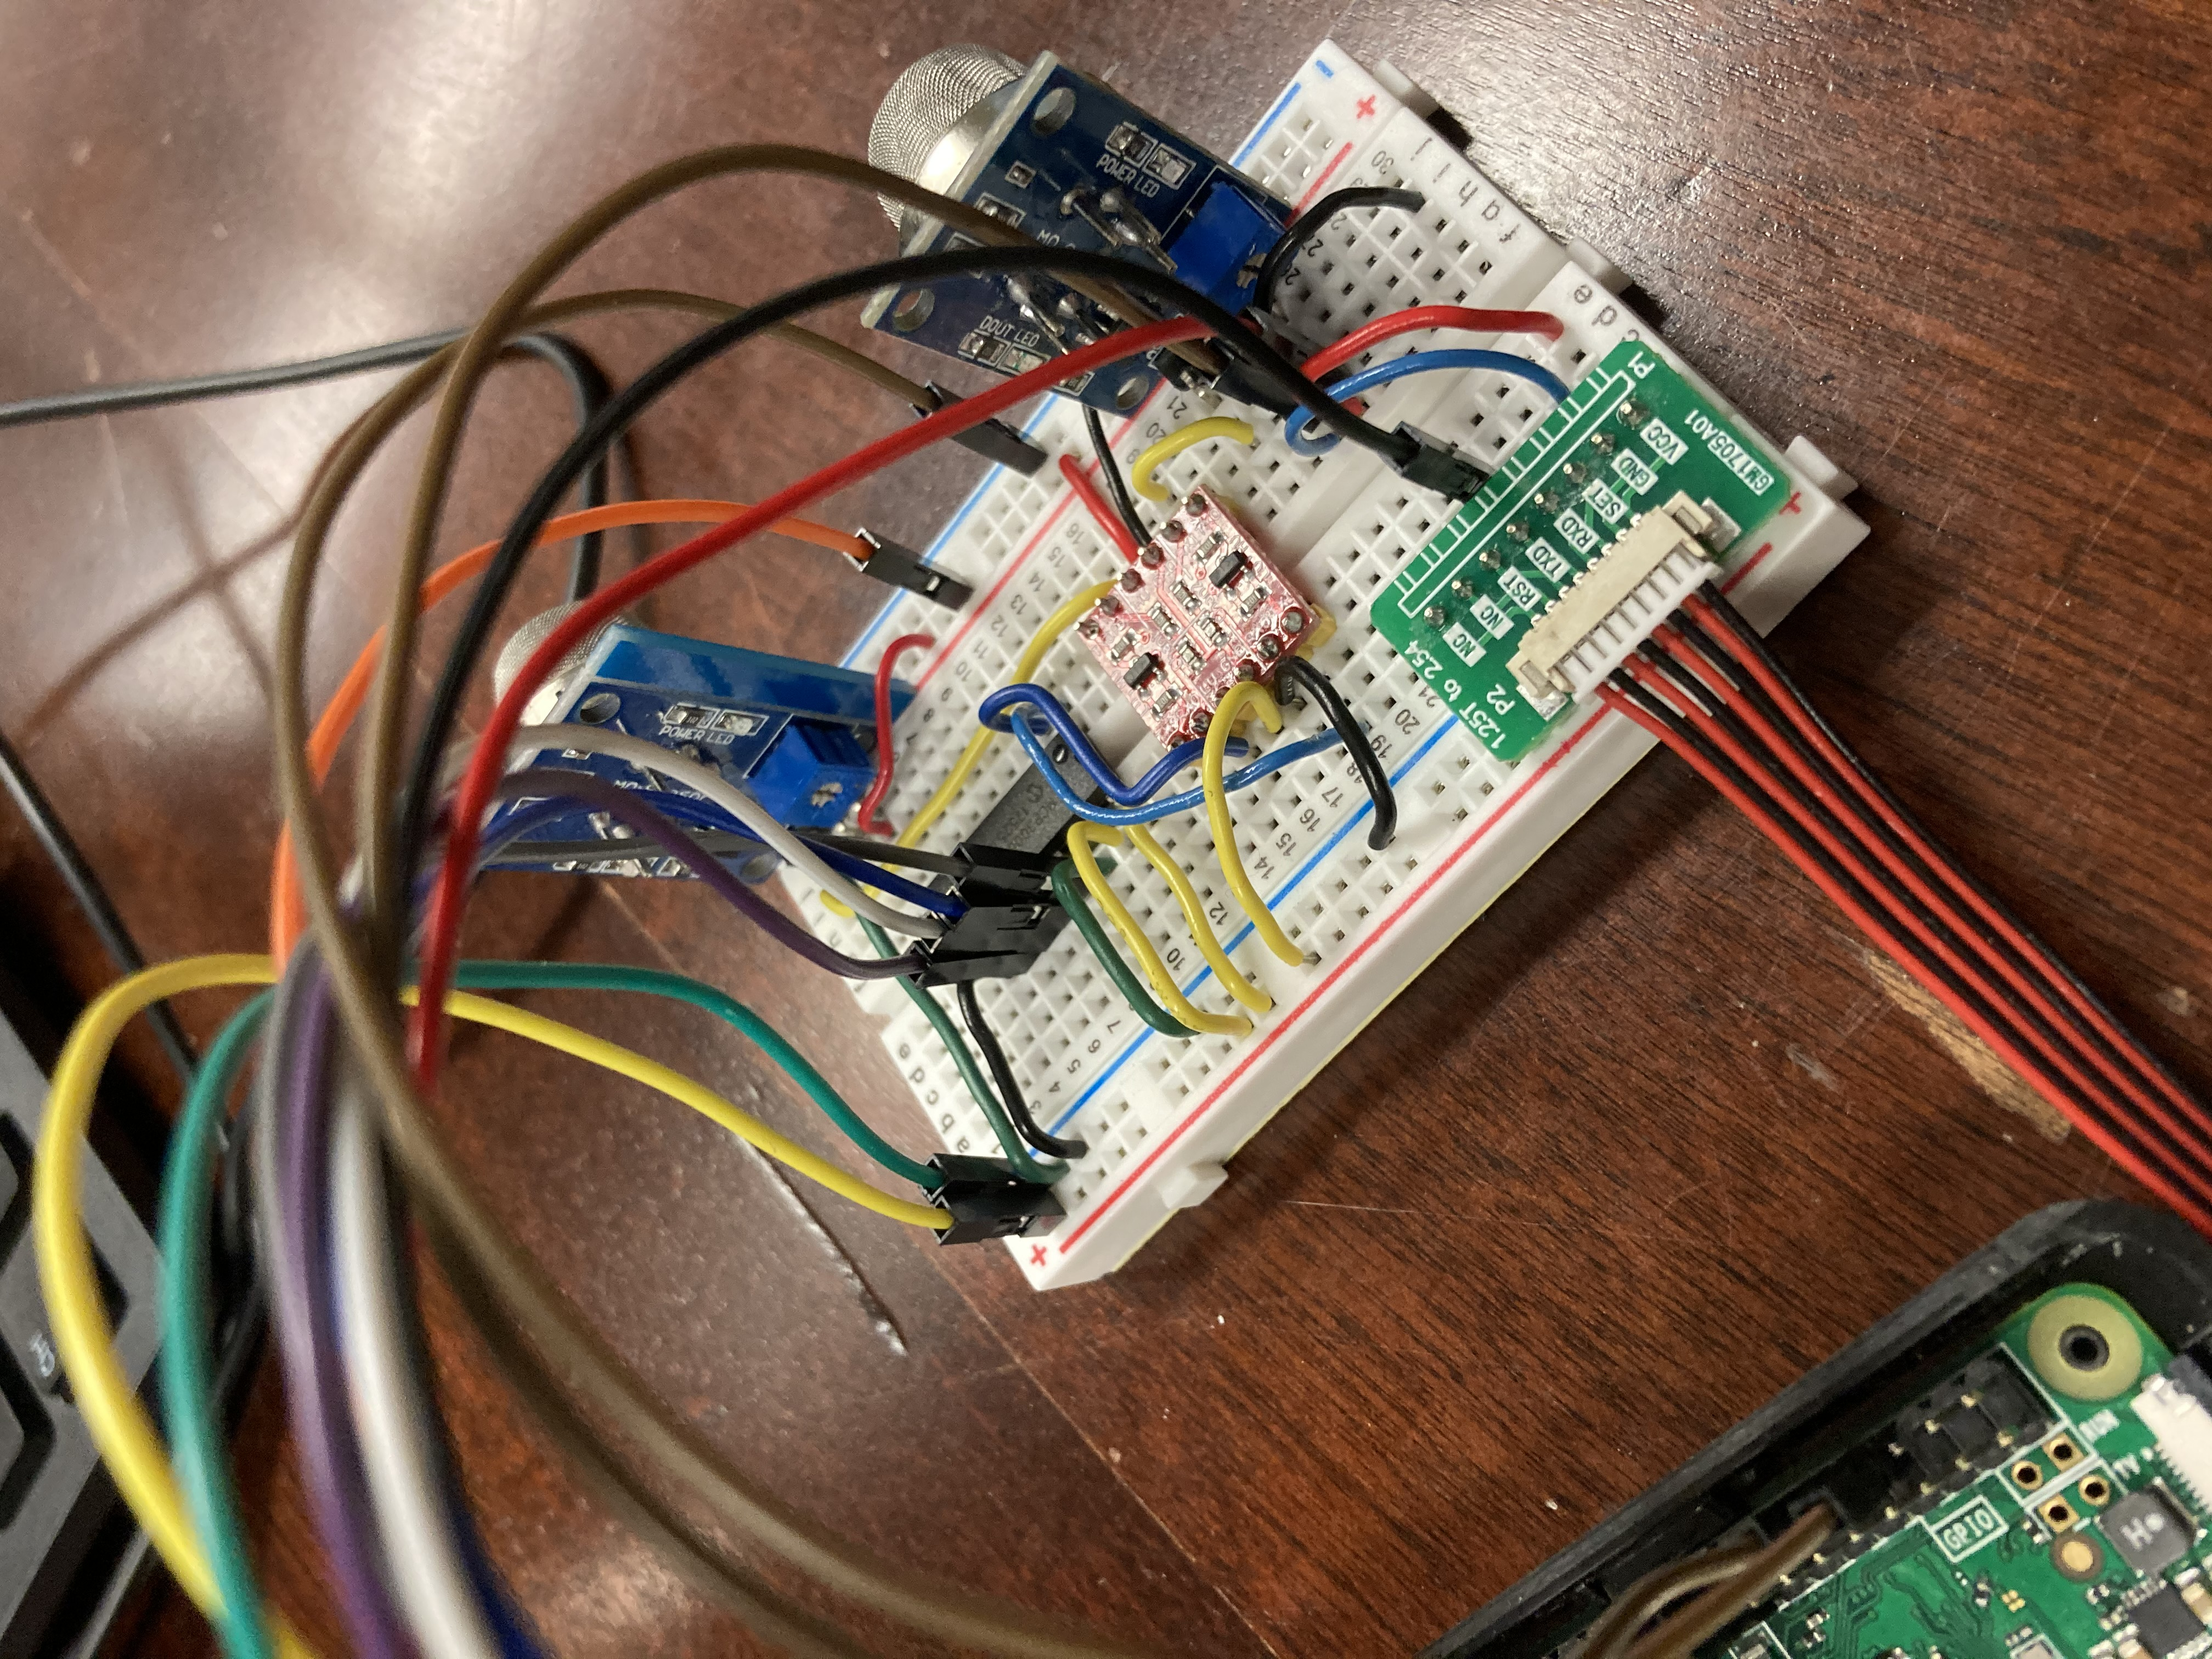
\includegraphics[width=1.00\textwidth]{2_Breadboard_side.JPG}
\end{figure}

\begin{figure}
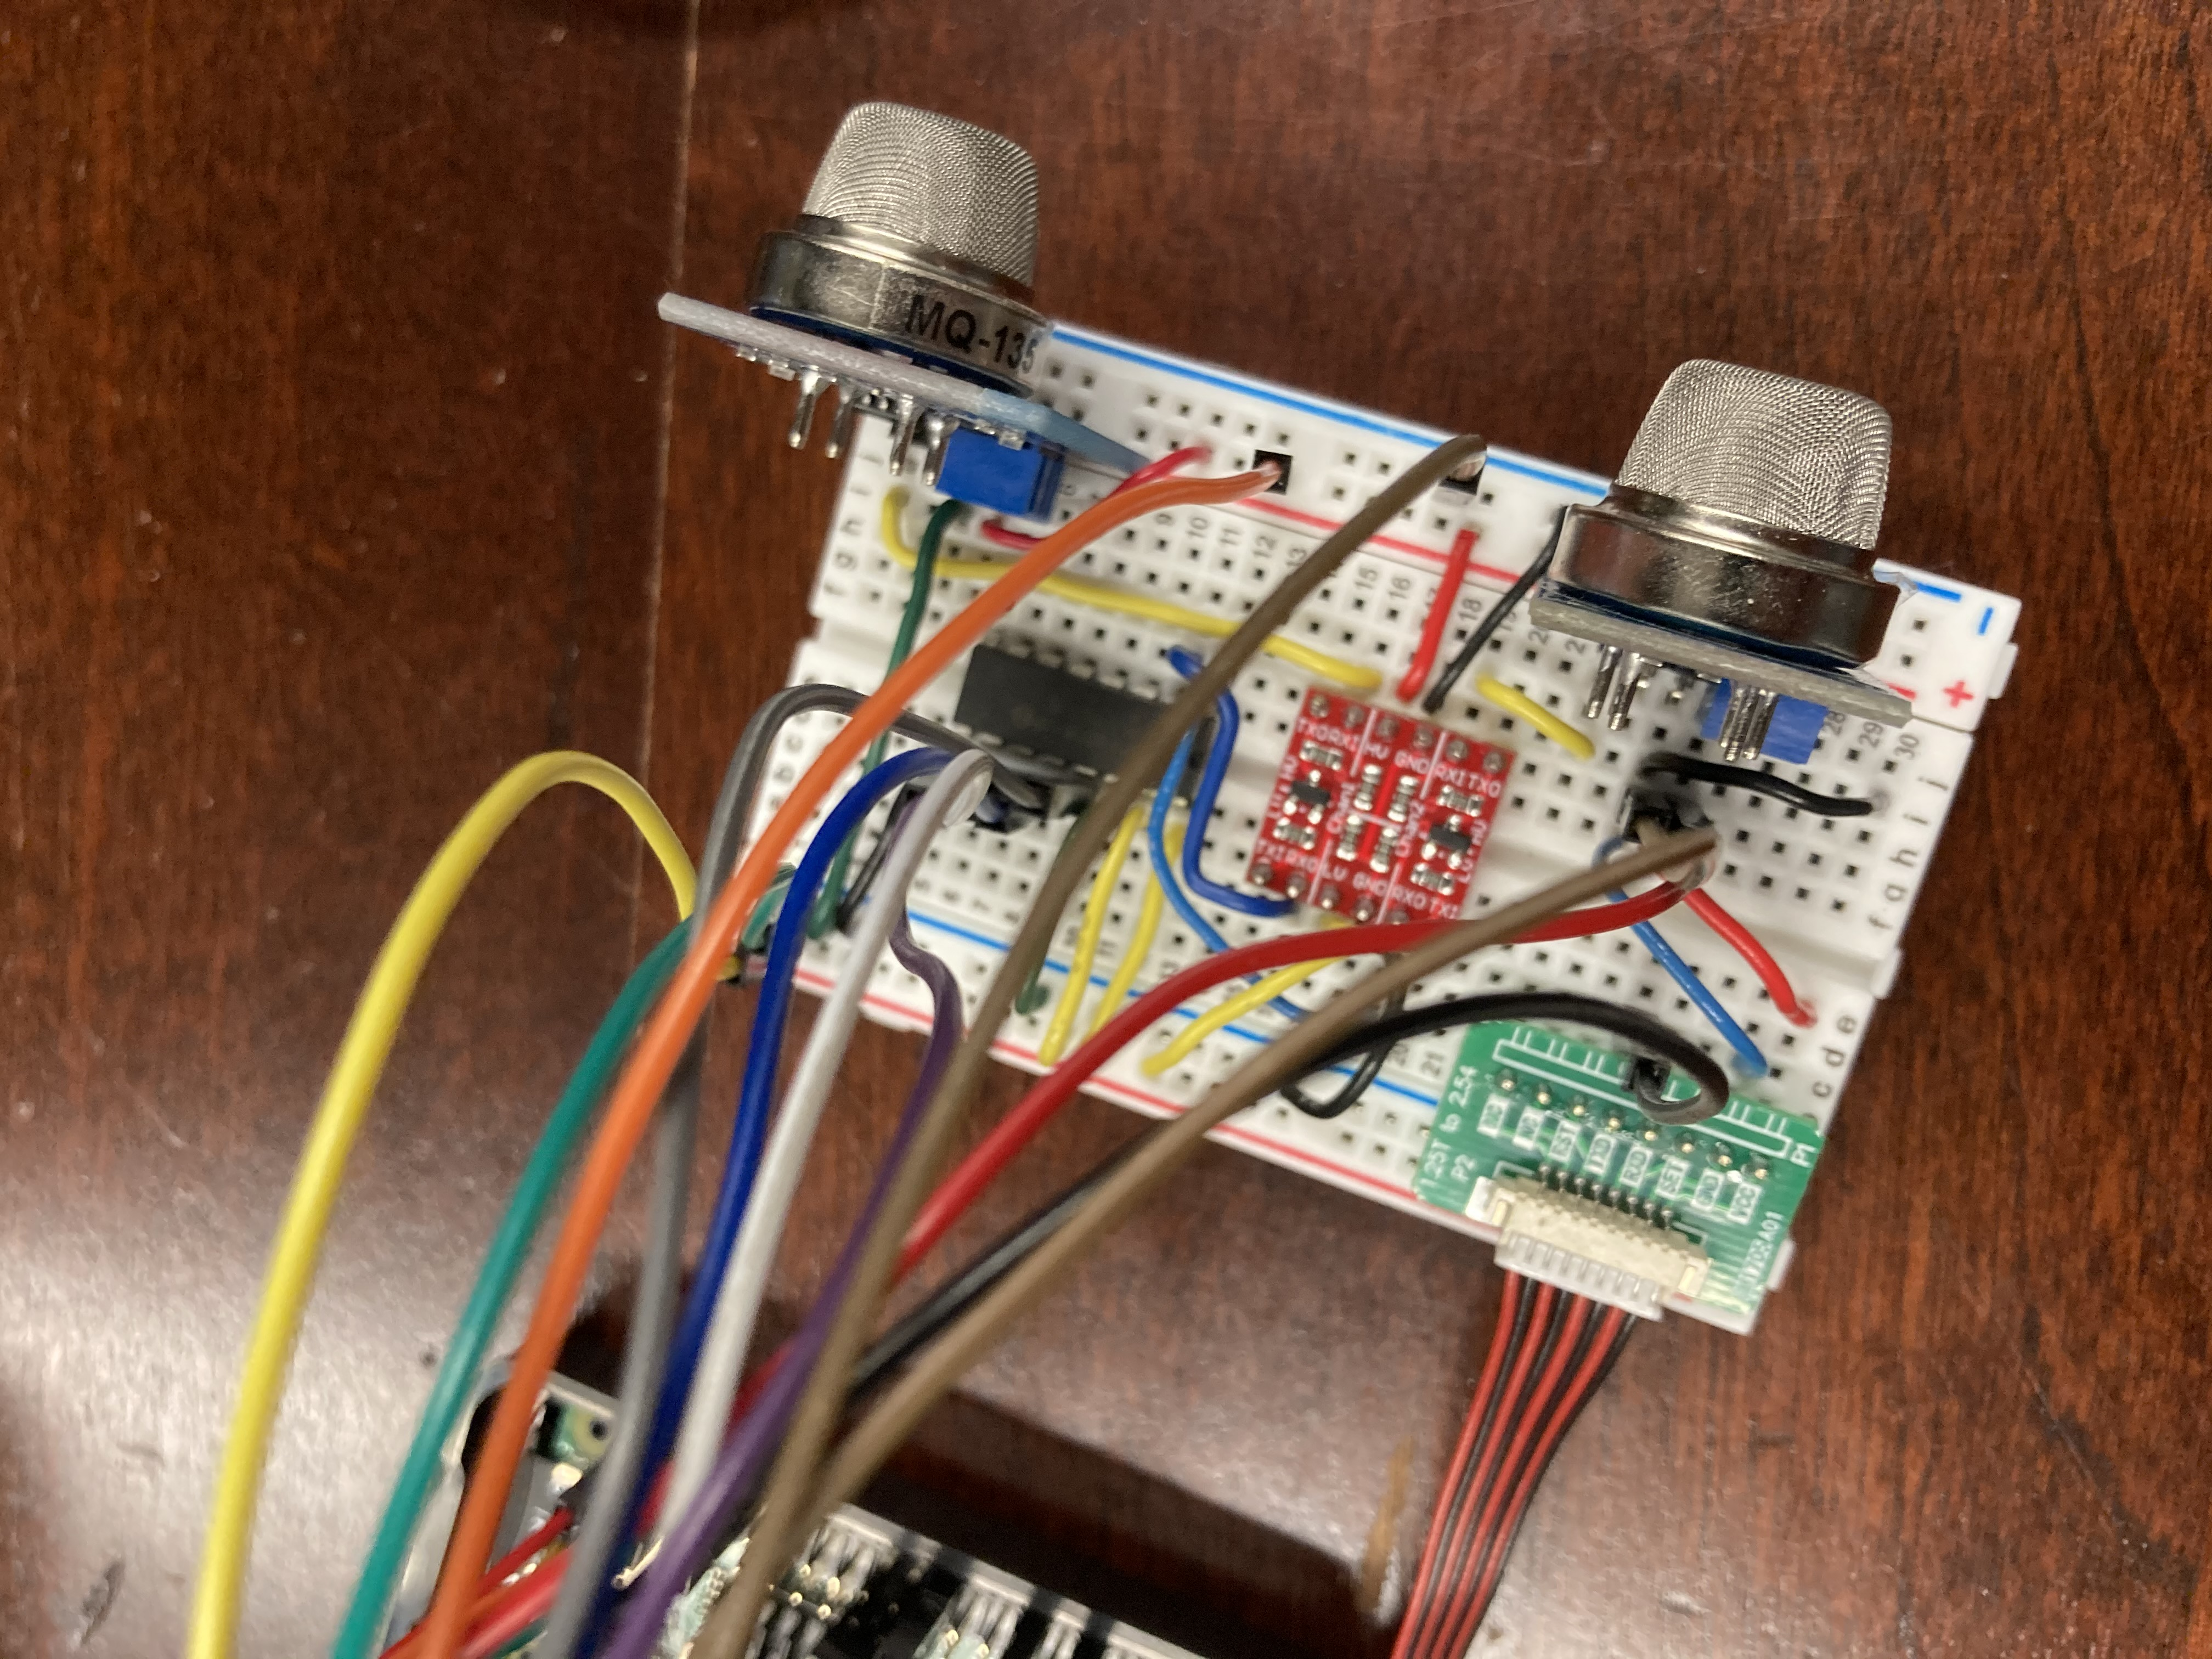
\includegraphics[width=1.00\textwidth]{2_Breadboard_all.JPG}
\end{figure}

\begin{figure}
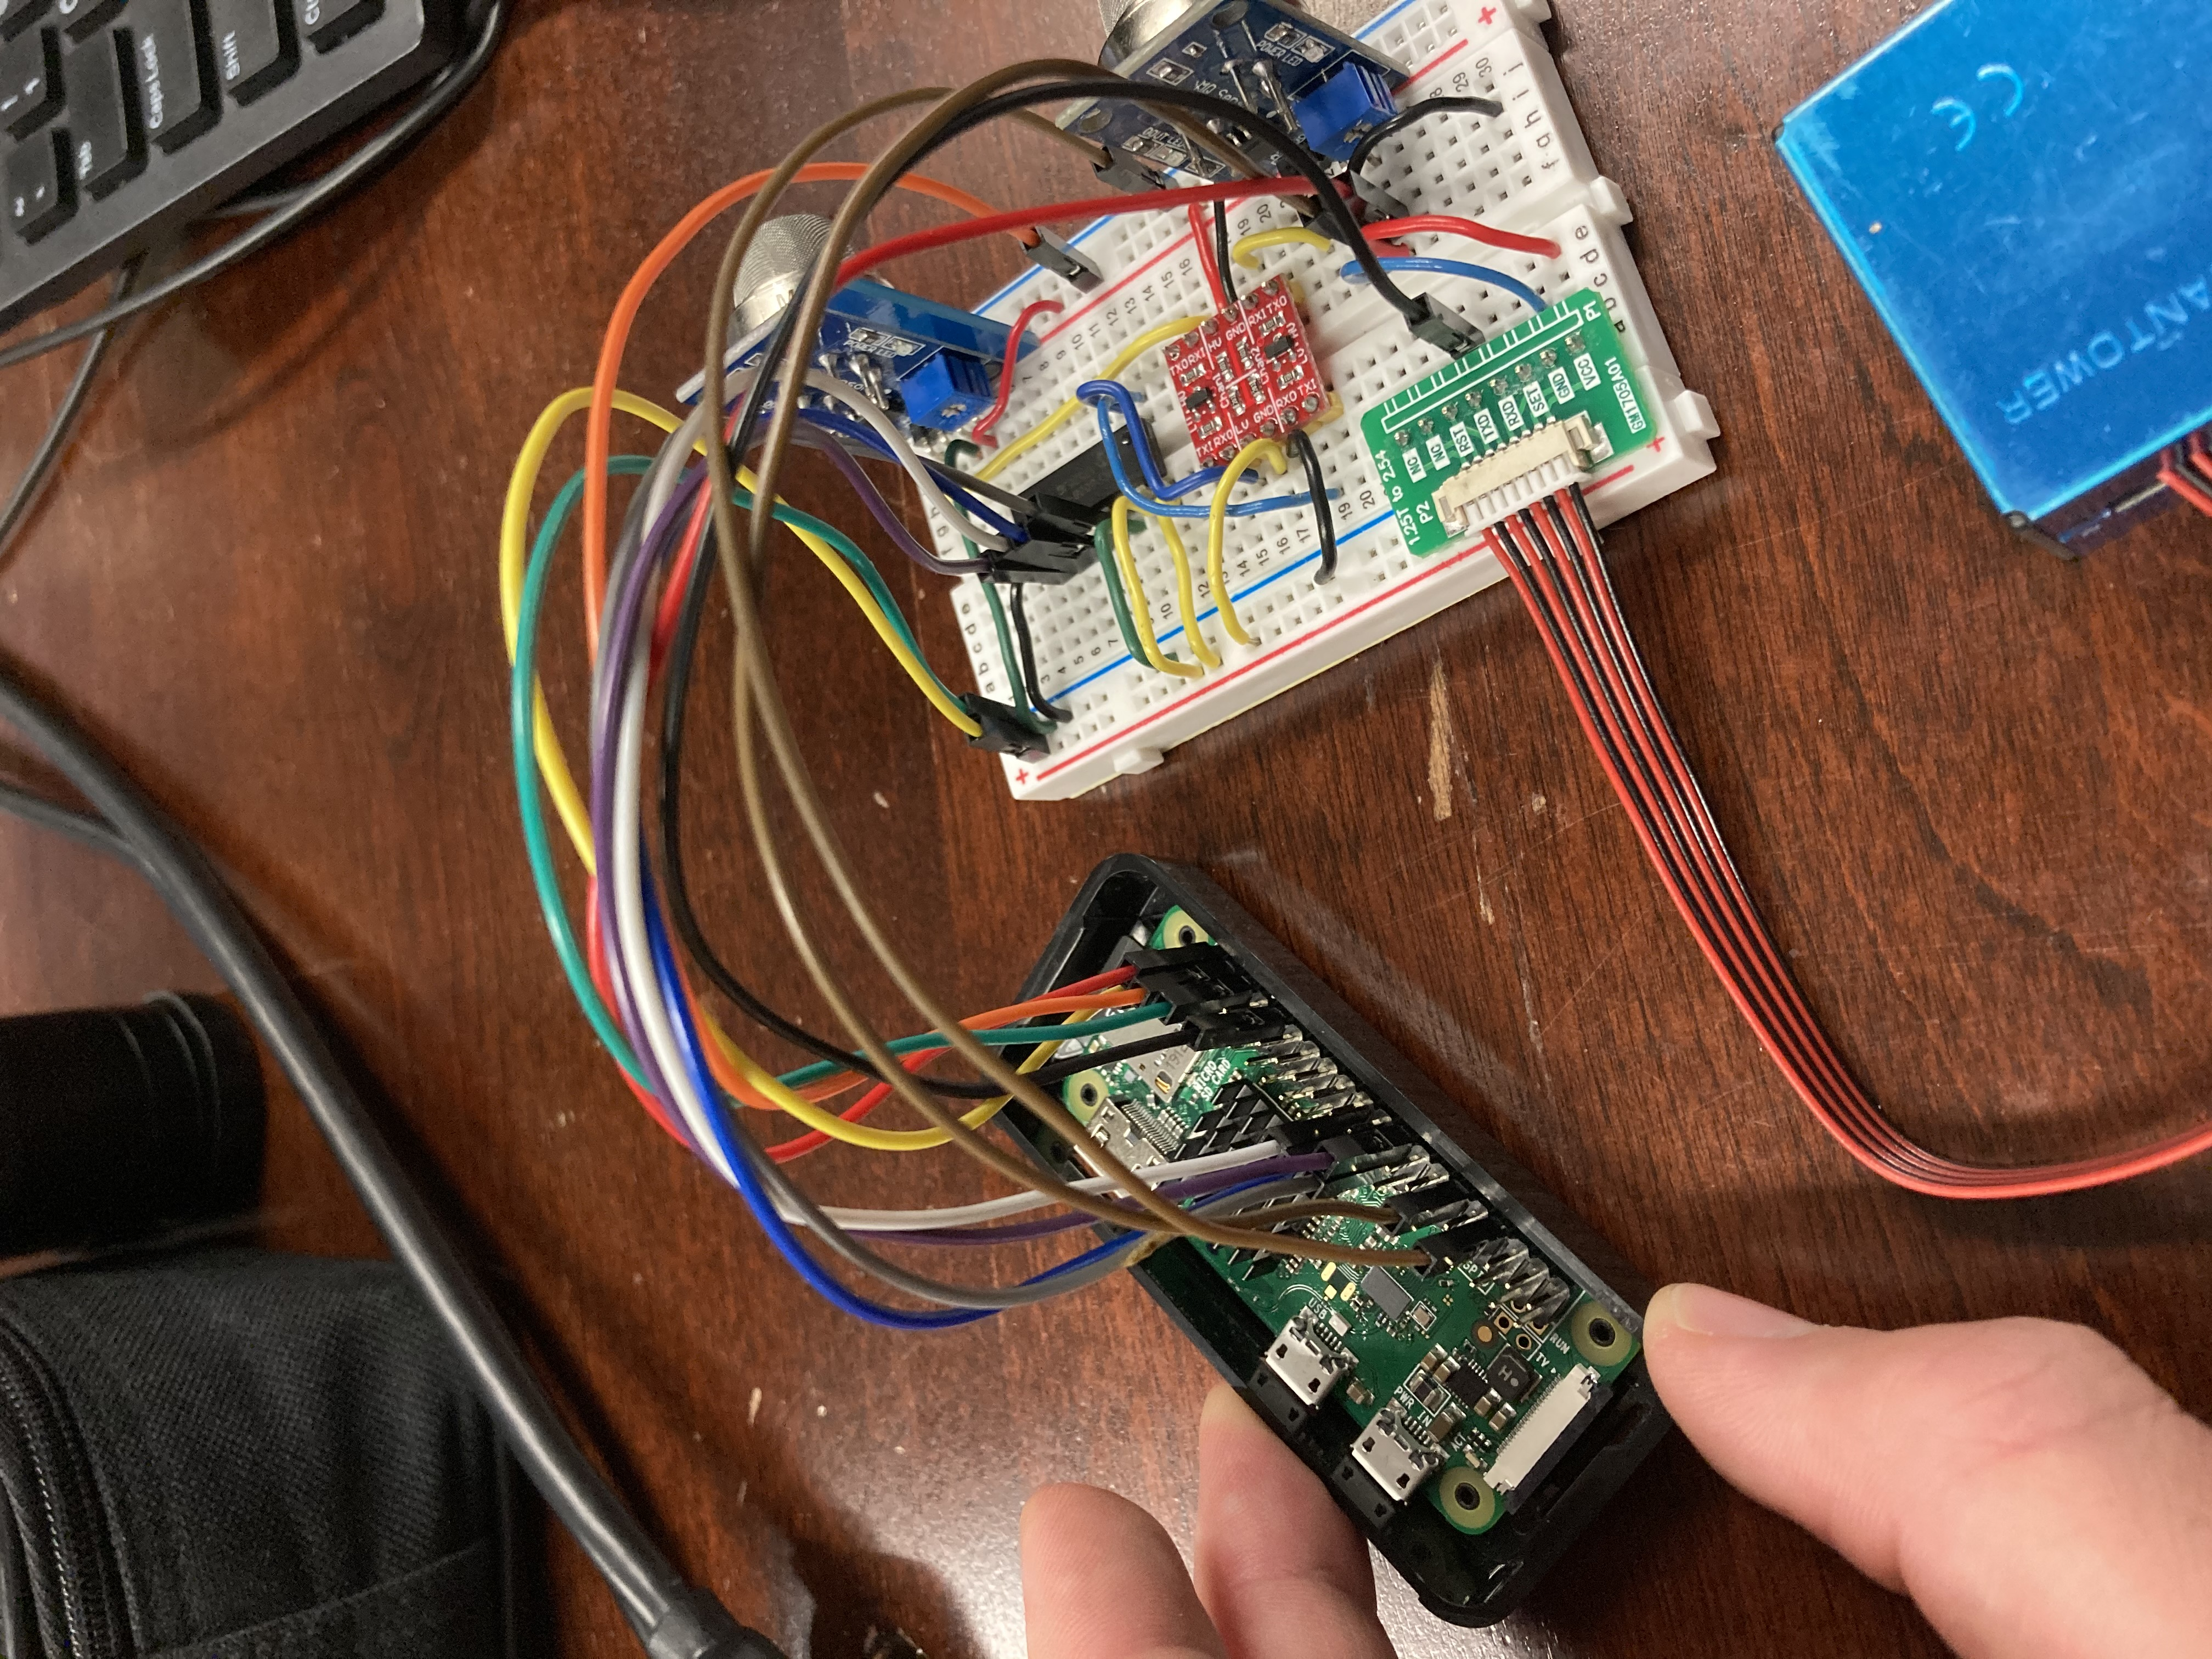
\includegraphics[width=1.00\textwidth]{2_Overview.JPG}
\end{figure}

\begin{figure}
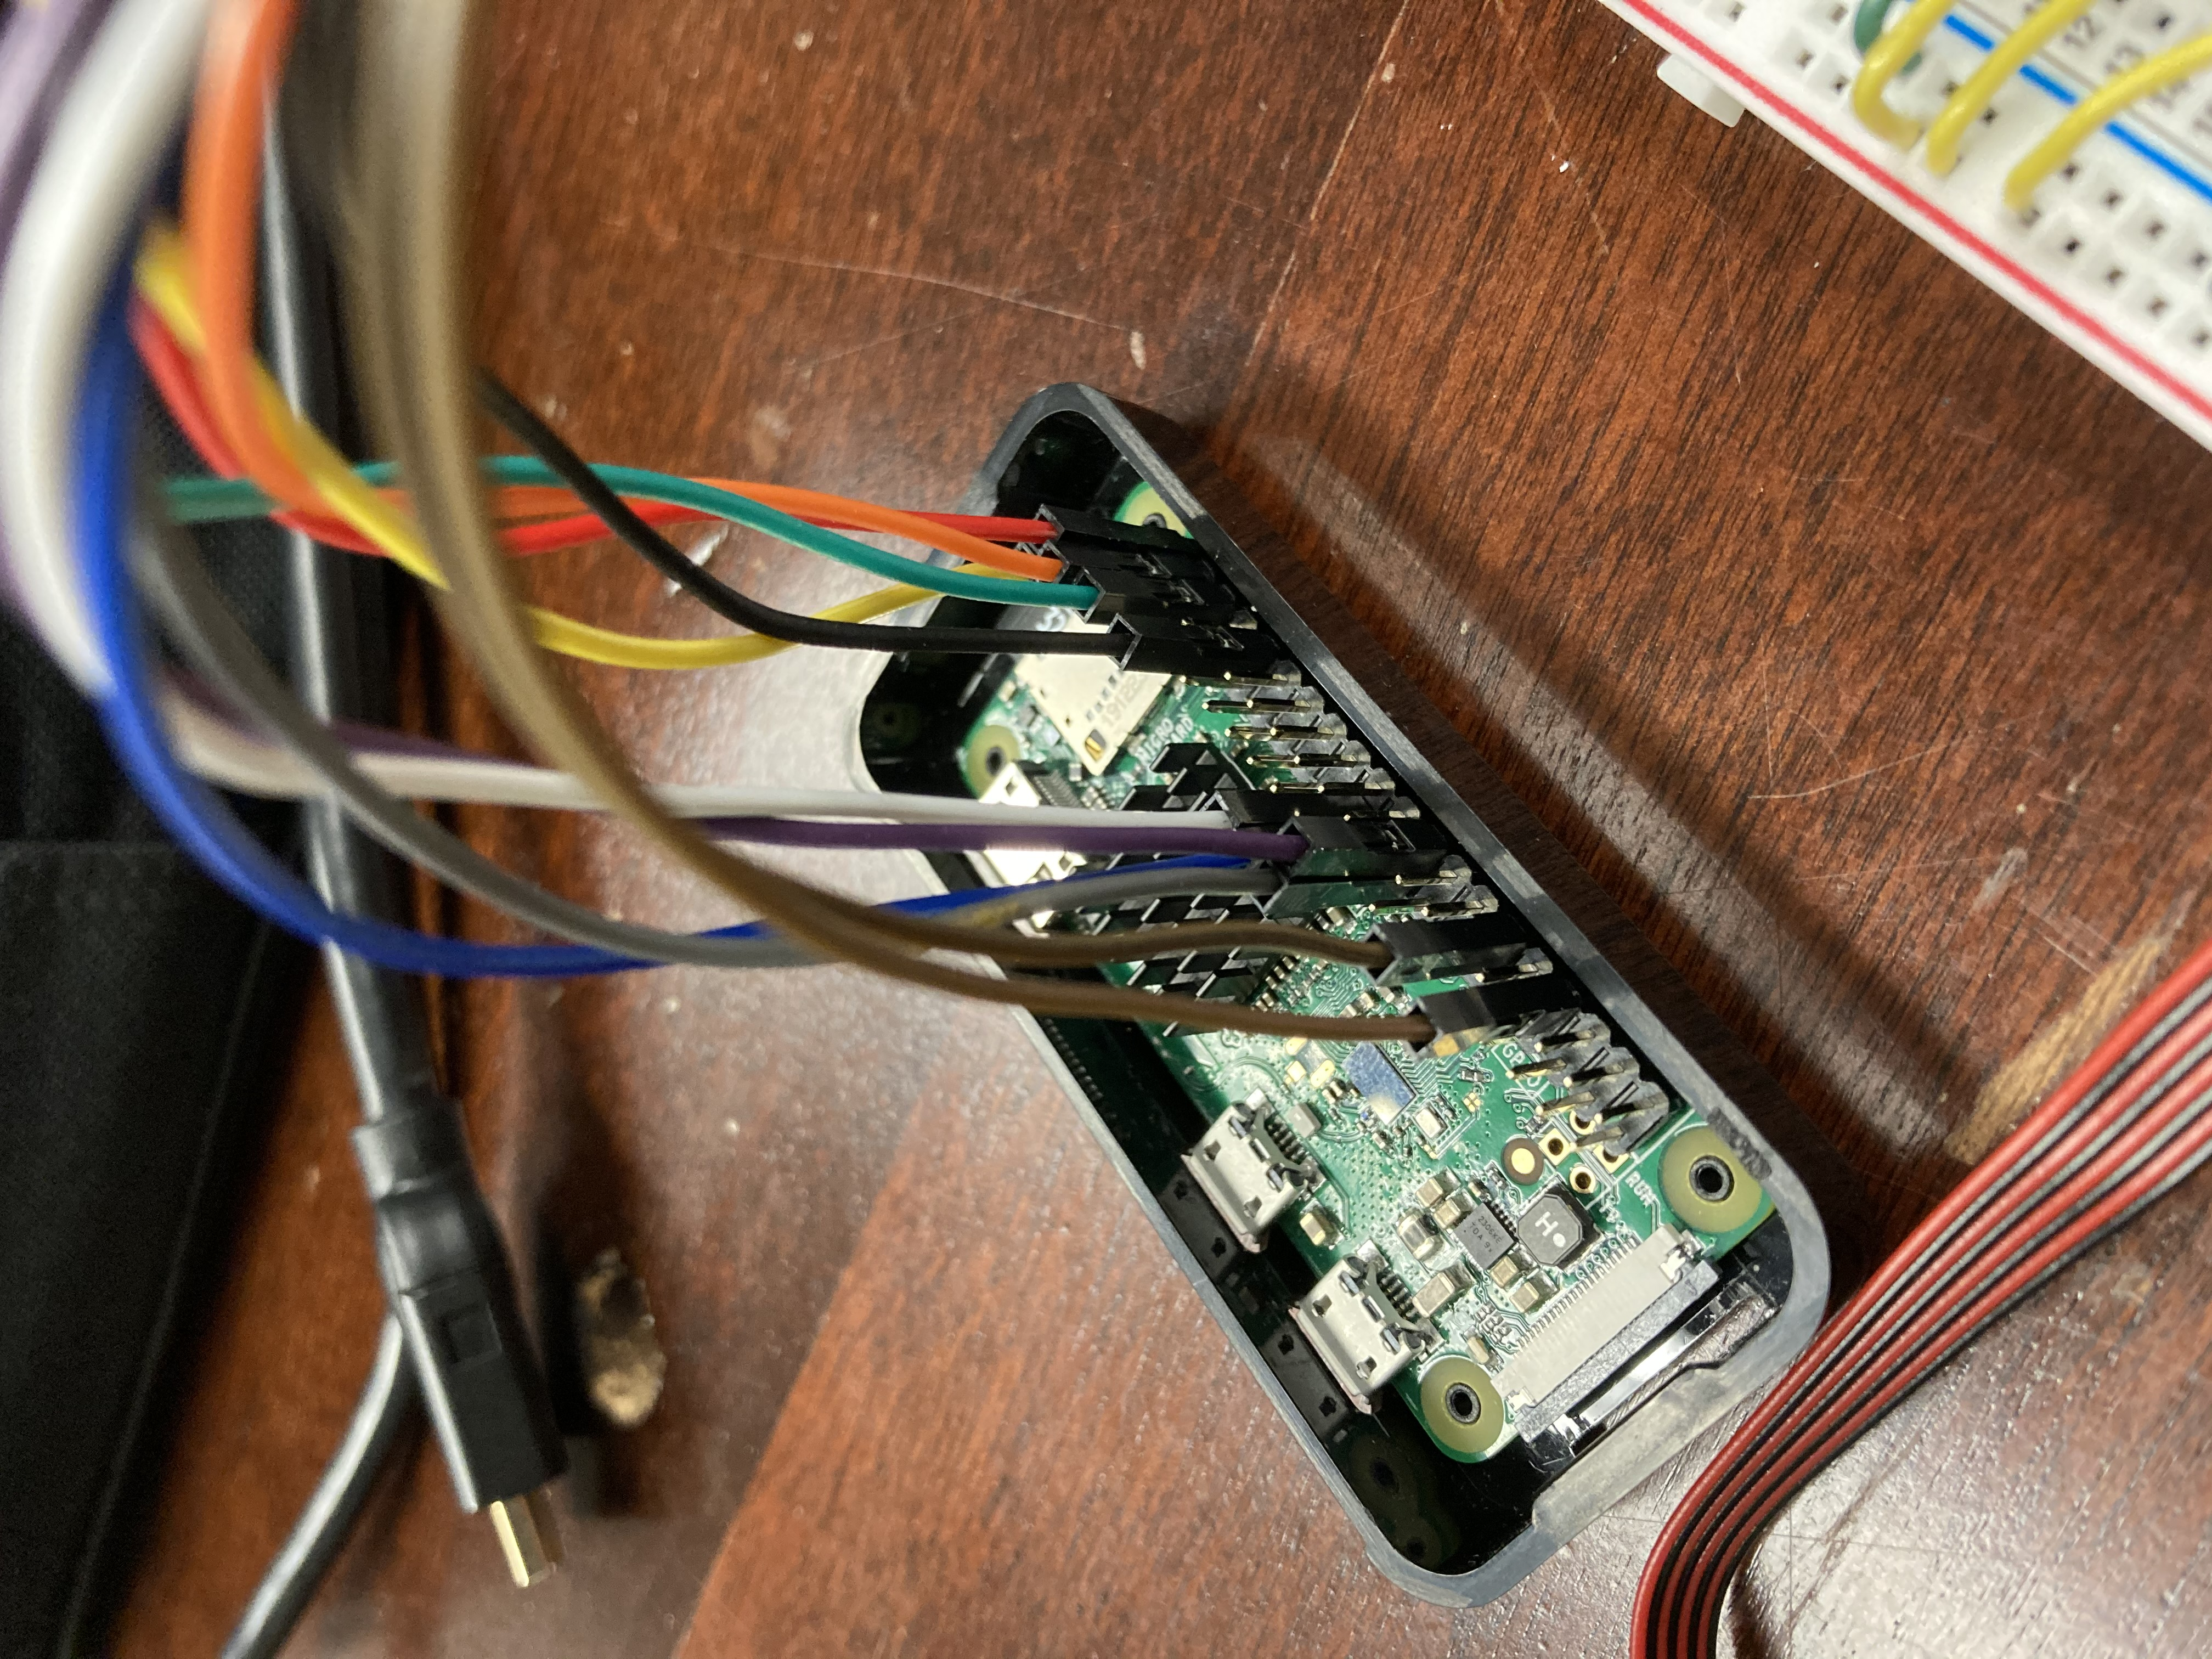
\includegraphics[width=1.00\textwidth]{2_Pi_Side.JPG}
\end{figure}

\begin{figure}
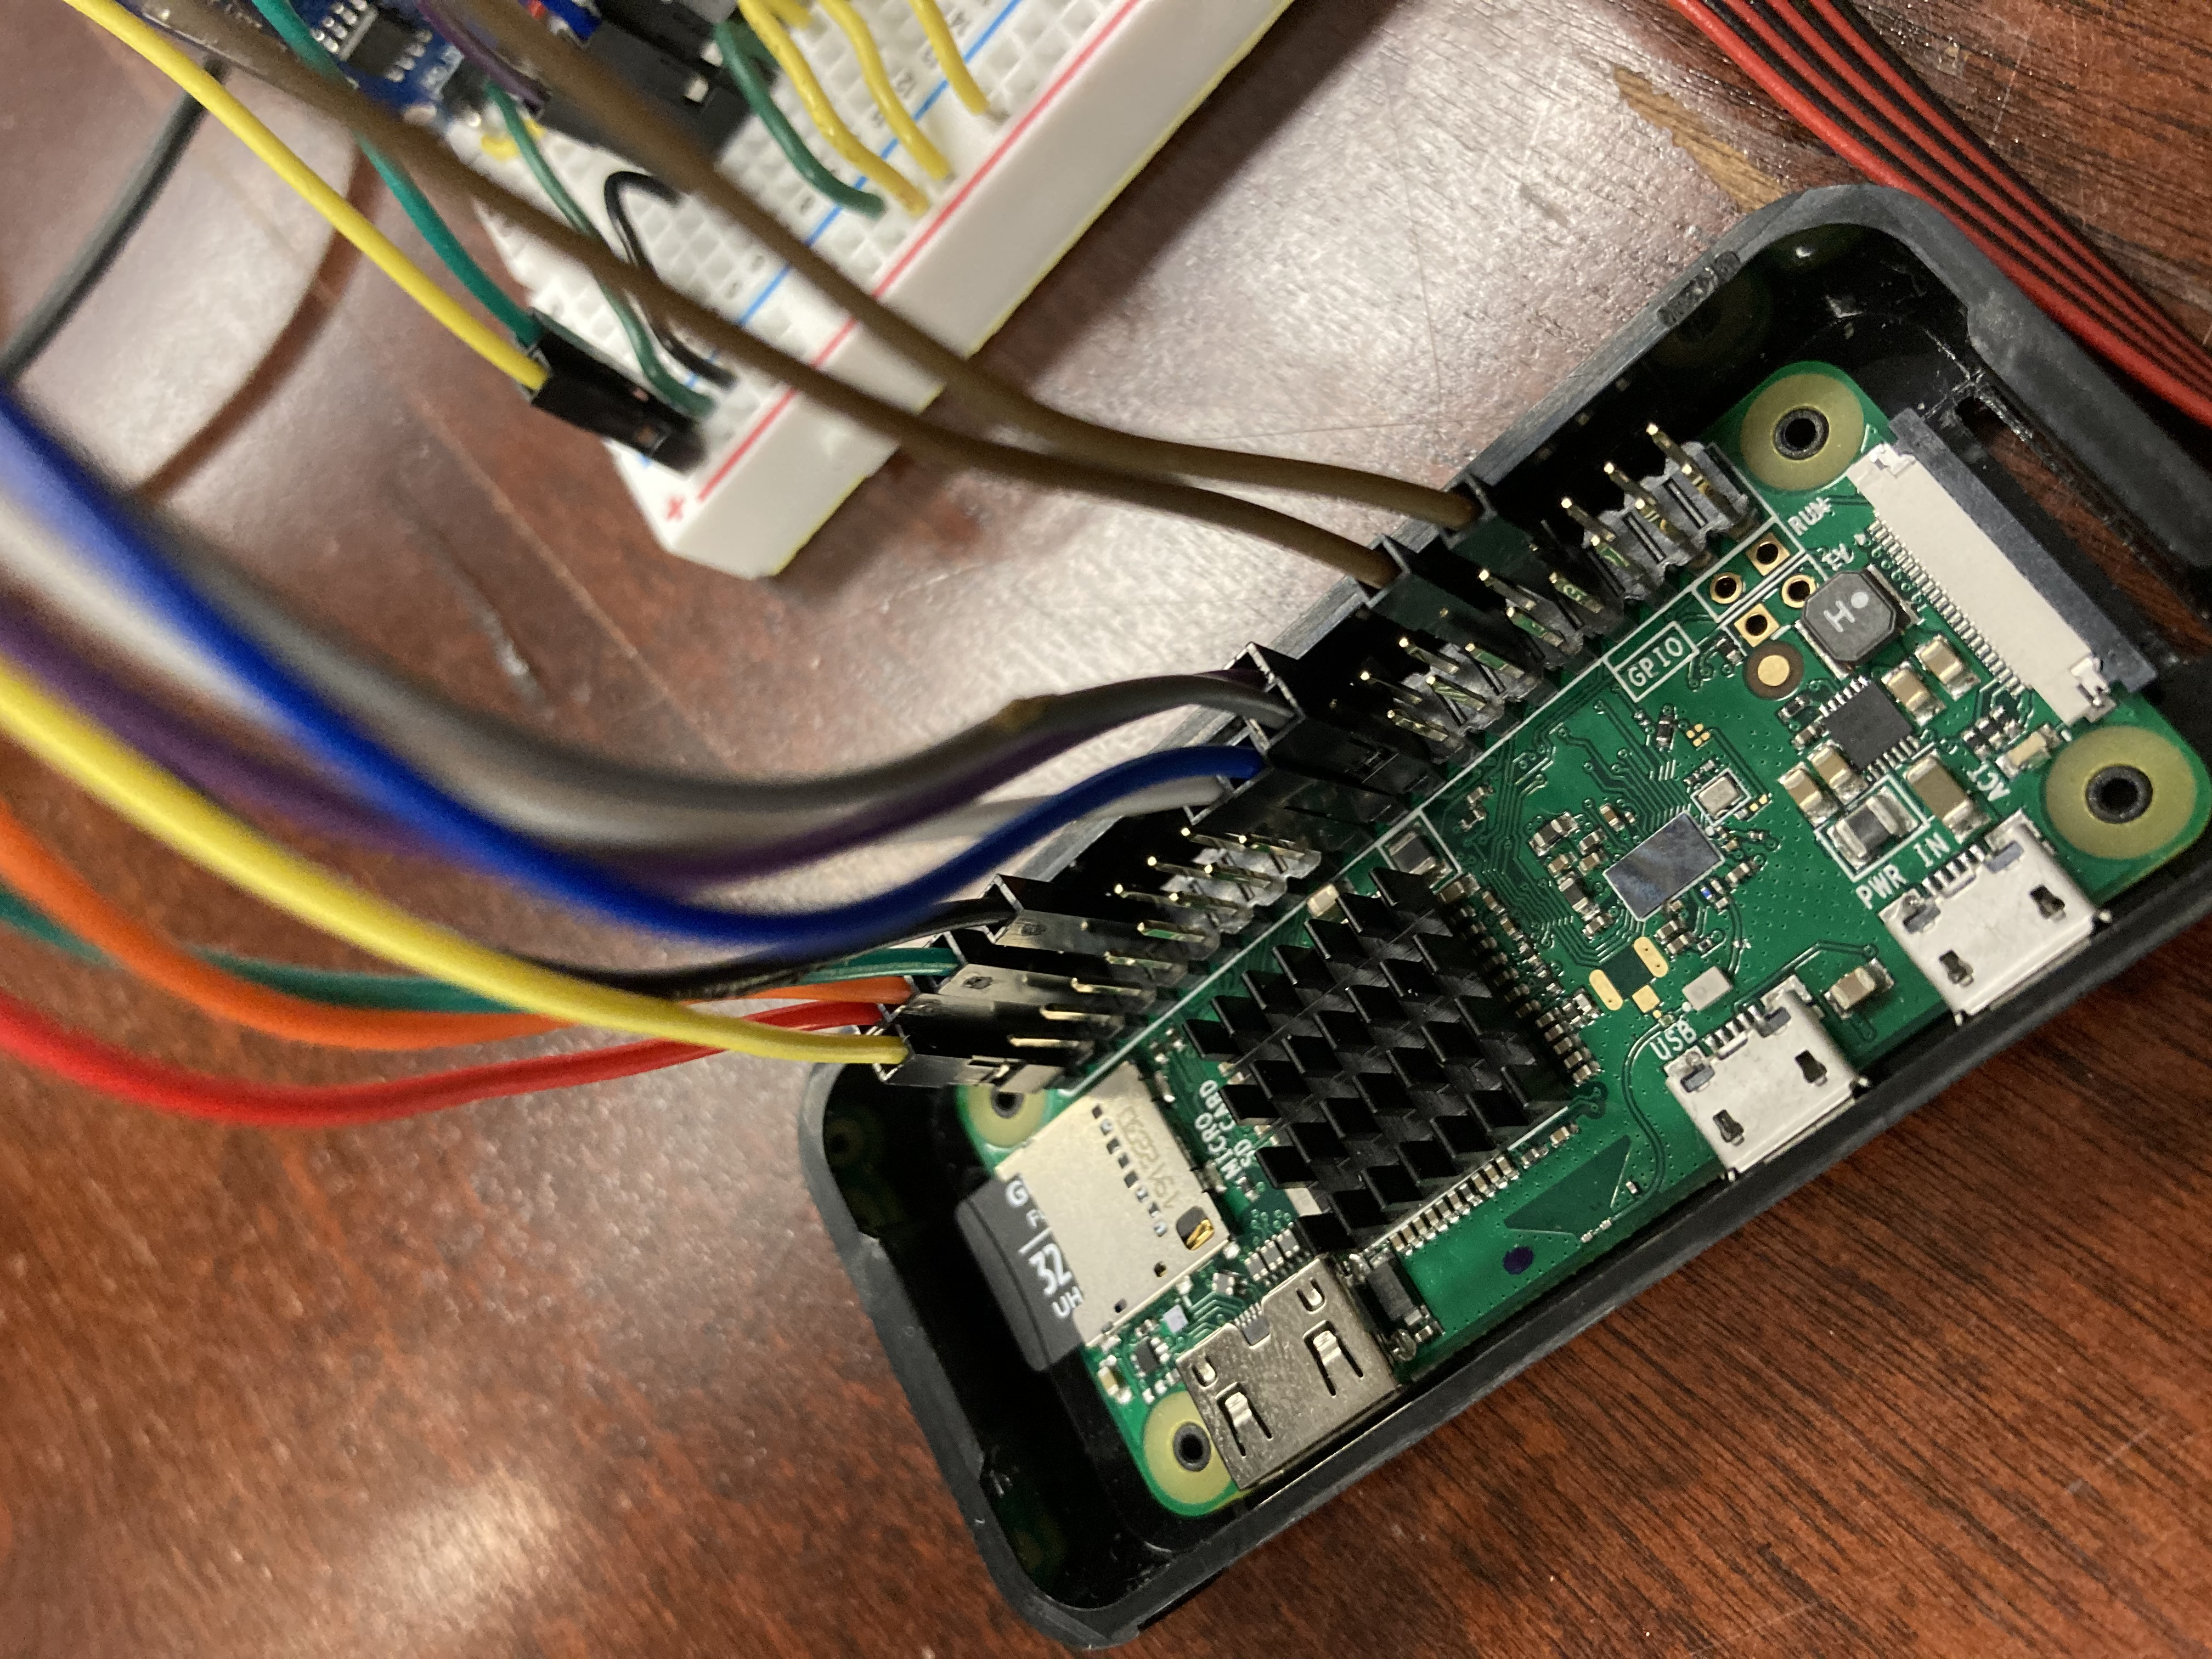
\includegraphics[width=1.00\textwidth]{2_Pi_overhead.JPG}
\end{figure}

\end{document}
